\icode[magenta]{E-MM-MU-L4-261014-001}
如图所示，两个均可视为质点的小球\(A\)、\(B\)用长为\(L\)的轻质细绳连接，\(B\)球穿在水平固定的光滑细杆上，小球\(A\)的质量为\(m\)，小球\(B\)的质量为\(3m\)。初始时细绳处于水平状态，现将两小球由静止释放，小球\(A\)在竖直平面内摆动的轨迹为如图所示的半椭圆。已知半长轴为\(a\)、半短轴为\(b\)的椭圆在最低点的曲率半径\(\rho = \frac{b^2}{a}\)，向心加速度大小\(a_{\text{向}}= \frac{v^2}{\rho}\)，不计空气阻力，重力加速度大小为g。下列说法正确的是\paren[]
	
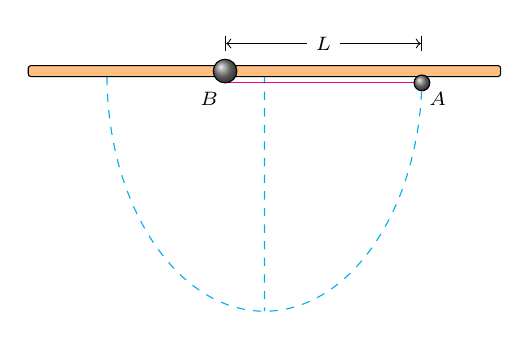
\begin{tikzpicture}[font=\scriptsize]
	\draw[dashed,cyan] (2,0) arc(0:-180:2 and 3) (0,0)--(0,-3);
	\draw[rounded corners=1,fill=orange!50] (-3,-.02) rectangle(3,.12);
    \draw[magenta] (-.5,-.1)--(2,-.1);
	\draw[ball color=gray] (-.5,.05) circle(.15);
	\draw[ball color=gray] (2,-.1) circle(.1);
	\draw[|<->|] (-0.5,.4)--node[fill=white]{\(L\)}(2,.4);
	\node at(-.7,-.1)[below]{\(B\)};
	\node at(2.2,-.1)[below]{\(A\)};
\end{tikzpicture}
\begin{choices}
	\item 图中椭圆的半短轴为\(\frac{3L}{4}\)
	\item 小球\(B\)的最大速度为\(\frac{\sqrt{6gl}}{6}\)
	\item 小球\(A\)到达最低点时的速度大小为\(\frac{\sqrt{6gl}}{3}\)
	\item 小球\(A\)到达最低点时细绳中的张力大小为\(\frac{11mg}{3}\)
\end{choices}
\begin{answer}
   ABD\qquad 提示： 
\end{answer}